% Options for packages loaded elsewhere
% Options for packages loaded elsewhere
\PassOptionsToPackage{unicode}{hyperref}
\PassOptionsToPackage{hyphens}{url}
\PassOptionsToPackage{dvipsnames,svgnames,x11names}{xcolor}
%
\documentclass[
  letterpaper,
  DIV=11,
  numbers=noendperiod]{scrartcl}
\usepackage{xcolor}
\usepackage[margin=1in]{geometry}
\usepackage{amsmath,amssymb}
\setcounter{secnumdepth}{5}
\usepackage{iftex}
\ifPDFTeX
  \usepackage[T1]{fontenc}
  \usepackage[utf8]{inputenc}
  \usepackage{textcomp} % provide euro and other symbols
\else % if luatex or xetex
  \usepackage{unicode-math} % this also loads fontspec
  \defaultfontfeatures{Scale=MatchLowercase}
  \defaultfontfeatures[\rmfamily]{Ligatures=TeX,Scale=1}
\fi
\usepackage{lmodern}
\ifPDFTeX\else
  % xetex/luatex font selection
\fi
% Use upquote if available, for straight quotes in verbatim environments
\IfFileExists{upquote.sty}{\usepackage{upquote}}{}
\IfFileExists{microtype.sty}{% use microtype if available
  \usepackage[]{microtype}
  \UseMicrotypeSet[protrusion]{basicmath} % disable protrusion for tt fonts
}{}
\makeatletter
\@ifundefined{KOMAClassName}{% if non-KOMA class
  \IfFileExists{parskip.sty}{%
    \usepackage{parskip}
  }{% else
    \setlength{\parindent}{0pt}
    \setlength{\parskip}{6pt plus 2pt minus 1pt}}
}{% if KOMA class
  \KOMAoptions{parskip=half}}
\makeatother
% Make \paragraph and \subparagraph free-standing
\makeatletter
\ifx\paragraph\undefined\else
  \let\oldparagraph\paragraph
  \renewcommand{\paragraph}{
    \@ifstar
      \xxxParagraphStar
      \xxxParagraphNoStar
  }
  \newcommand{\xxxParagraphStar}[1]{\oldparagraph*{#1}\mbox{}}
  \newcommand{\xxxParagraphNoStar}[1]{\oldparagraph{#1}\mbox{}}
\fi
\ifx\subparagraph\undefined\else
  \let\oldsubparagraph\subparagraph
  \renewcommand{\subparagraph}{
    \@ifstar
      \xxxSubParagraphStar
      \xxxSubParagraphNoStar
  }
  \newcommand{\xxxSubParagraphStar}[1]{\oldsubparagraph*{#1}\mbox{}}
  \newcommand{\xxxSubParagraphNoStar}[1]{\oldsubparagraph{#1}\mbox{}}
\fi
\makeatother


\usepackage{longtable,booktabs,array}
\newcounter{none} % for unnumbered tables
\usepackage{calc} % for calculating minipage widths
% Correct order of tables after \paragraph or \subparagraph
\usepackage{etoolbox}
\makeatletter
\patchcmd\longtable{\par}{\if@noskipsec\mbox{}\fi\par}{}{}
\makeatother
% Allow footnotes in longtable head/foot
\IfFileExists{footnotehyper.sty}{\usepackage{footnotehyper}}{\usepackage{footnote}}
\makesavenoteenv{longtable}
\usepackage{graphicx}
\makeatletter
\newsavebox\pandoc@box
\newcommand*\pandocbounded[1]{% scales image to fit in text height/width
  \sbox\pandoc@box{#1}%
  \Gscale@div\@tempa{\textheight}{\dimexpr\ht\pandoc@box+\dp\pandoc@box\relax}%
  \Gscale@div\@tempb{\linewidth}{\wd\pandoc@box}%
  \ifdim\@tempb\p@<\@tempa\p@\let\@tempa\@tempb\fi% select the smaller of both
  \ifdim\@tempa\p@<\p@\scalebox{\@tempa}{\usebox\pandoc@box}%
  \else\usebox{\pandoc@box}%
  \fi%
}
% Set default figure placement to htbp
\def\fps@figure{htbp}
\makeatother


% definitions for citeproc citations
\NewDocumentCommand\citeproctext{}{}
\NewDocumentCommand\citeproc{mm}{%
  \begingroup\def\citeproctext{#2}\cite{#1}\endgroup}
\makeatletter
 % allow citations to break across lines
 \let\@cite@ofmt\@firstofone
 % avoid brackets around text for \cite:
 \def\@biblabel#1{}
 \def\@cite#1#2{{#1\if@tempswa , #2\fi}}
\makeatother
\newlength{\cslhangindent}
\setlength{\cslhangindent}{1.5em}
\newlength{\csllabelwidth}
\setlength{\csllabelwidth}{3em}
\newenvironment{CSLReferences}[2] % #1 hanging-indent, #2 entry-spacing
 {\begin{list}{}{%
  \setlength{\itemindent}{0pt}
  \setlength{\leftmargin}{0pt}
  \setlength{\parsep}{0pt}
  % turn on hanging indent if param 1 is 1
  \ifodd #1
   \setlength{\leftmargin}{\cslhangindent}
   \setlength{\itemindent}{-1\cslhangindent}
  \fi
  % set entry spacing
  \setlength{\itemsep}{#2\baselineskip}}}
 {\end{list}}
\usepackage{calc}
\newcommand{\CSLBlock}[1]{\hfill\break\parbox[t]{\linewidth}{\strut\ignorespaces#1\strut}}
\newcommand{\CSLLeftMargin}[1]{\parbox[t]{\csllabelwidth}{\strut#1\strut}}
\newcommand{\CSLRightInline}[1]{\parbox[t]{\linewidth - \csllabelwidth}{\strut#1\strut}}
\newcommand{\CSLIndent}[1]{\hspace{\cslhangindent}#1}



\setlength{\emergencystretch}{3em} % prevent overfull lines

\providecommand{\tightlist}{%
  \setlength{\itemsep}{0pt}\setlength{\parskip}{0pt}}



 


\usepackage{booktabs}
\usepackage{longtable}
\usepackage{array}
\usepackage{multirow}
\usepackage{wrapfig}
\usepackage{float}
\usepackage{colortbl}
\usepackage{pdflscape}
\usepackage{tabularx}
\usepackage{xltabular}
\usepackage{threeparttable}
\usepackage{threeparttablex}
\usepackage[normalem]{ulem}
\usepackage{makecell}
\usepackage{xcolor}
\usepackage{caption}
\usepackage{anyfontsize}
\usepackage{placeins}
\usepackage{float}
\KOMAoption{captions}{tableheading}
\makeatletter
\@ifpackageloaded{caption}{}{\usepackage{caption}}
\AtBeginDocument{%
\ifdefined\contentsname
  \renewcommand*\contentsname{Table of contents}
\else
  \newcommand\contentsname{Table of contents}
\fi
\ifdefined\listfigurename
  \renewcommand*\listfigurename{List of Figures}
\else
  \newcommand\listfigurename{List of Figures}
\fi
\ifdefined\listtablename
  \renewcommand*\listtablename{List of Tables}
\else
  \newcommand\listtablename{List of Tables}
\fi
\ifdefined\figurename
  \renewcommand*\figurename{Figure}
\else
  \newcommand\figurename{Figure}
\fi
\ifdefined\tablename
  \renewcommand*\tablename{Table}
\else
  \newcommand\tablename{Table}
\fi
}
\@ifpackageloaded{float}{}{\usepackage{float}}
\floatstyle{ruled}
\@ifundefined{c@chapter}{\newfloat{codelisting}{h}{lop}}{\newfloat{codelisting}{h}{lop}[chapter]}
\floatname{codelisting}{Listing}
\newcommand*\listoflistings{\listof{codelisting}{List of Listings}}
\makeatother
\makeatletter
\makeatother
\makeatletter
\@ifpackageloaded{caption}{}{\usepackage{caption}}
\@ifpackageloaded{subcaption}{}{\usepackage{subcaption}}
\makeatother
\usepackage{bookmark}
\IfFileExists{xurl.sty}{\usepackage{xurl}}{} % add URL line breaks if available
\urlstyle{same}
\hypersetup{
  pdftitle={North American Bat Monitoring Program in British Columbia},
  pdfauthor={Camila Hurtado; Taylor Hart},
  colorlinks=true,
  linkcolor={blue},
  filecolor={Maroon},
  citecolor={Blue},
  urlcolor={Blue},
  pdfcreator={LaTeX via pandoc}}


\title{North American Bat Monitoring Program in British Columbia}
\usepackage{etoolbox}
\makeatletter
\providecommand{\subtitle}[1]{% add subtitle to \maketitle
  \apptocmd{\@title}{\par {\large #1 \par}}{}{}
}
\makeatother
\subtitle{Data Summary and Activity Trend Analyses: 2016 - 2025}
\author{Camila Hurtado \and Taylor Hart}
\date{2026-09-28}
\begin{document}
\maketitle

\clearpage

\renewcommand*\contentsname{Table of contents}
{
\setcounter{tocdepth}{3}
\tableofcontents
}

\newpage{}

\section{Executive Summary}\label{executive-summary}

The North American Bat Monitoring (NABat) program is a multi-agency
initiative administered by the US Geological Survey (USGS). In 2024, the
North by Northwest (NNW) Bat Hub was formed by combining the former
Alberta Hub and the BC and Southeast Alaska (BC-SE\_AK) Hub. The NNW Bat
Hub leads the NABat program within British Columbia, with key support
from provincial and state representatives and WCSC. In 2025, 57 grid
cells throughout British Columbia were monitored. Results indicate that
bat populations across British Columbia remain stable, with some key
species showing small positive trends, including Little Brown Myotis and
Eastern Red Bat. Given growing threats to bat populations in BC,
continued monitoring is essential to detect any significant changes.

\section{Land Acknowledgement}\label{land-acknowledgement}

Biodiversity Pathways respectfully acknowledges that our work takes
place on Treaty 8 and Douglas Treaties Territories as well as the
traditional and unceded territories of First Nations and Métis Peoples
across all regions of British Columbia, whose histories, languages, and
cultures are deeply connected to the biodiversity we monitor. We
acknowledge the traditional teachings of the lands that we work on, and
that reciprocal, meaningful, and respectful relationships with
Indigenous peoples make our work possible. We are deeply grateful for
their stewardship of these lands, and we are committed to supporting
Indigenous-led monitoring programs, while learning Indigenous ways of
knowing, being, and doing.

\newpage{}

\section{Introduction}\label{introduction}

\subsection{Overview of NABat and the NNW Bat
Hub}\label{overview-of-nabat-and-the-nnw-bat-hub}

North American Bat Monitoring Program (NABat) is a large-scale
coordinated effort to monitor bat species to address gaps in knowledge
and lack of long-term studies across North America (Loeb et al.
2015).The program is administered by the US Geological Survey (USGS) and
implemented by the North by Northwest Bat (NNW) Hub in British Columbia,
Alberta and S.E Alaska.

NNW Bat Hub was established in 2024 with collaboration from Government
of British Columbia, Government of Alberta, and Government of Alaska.
The hub was formed by combining the previous Alberta Hub and the BC and
southeast Alaska (BC-SE\_AK) Hub. The implementation of the program
within British Columbia has key support from Wildlife Conservation
Society Canada (WCSC), government staff, other wildlife biologists,
Indigenous Nations, community members and naturalists across the
province.

The centralization of efforts for the hub will expand exciting programs
to coordinate more efficiently across jurisdictions, ensuring consistent
and long-term bat monitoring through standardized data collection, and
streamlined bioacoustic data management. It also seeks to enhance
engagement with NABat, foster collaboration among stakeholders, and
produce annual reports on regional monitoring.

\subsection{Threats to bat populations in
BC}\label{threats-to-bat-populations-in-bc}

Bat populations in British Columbia face a wide range of threats
including forestry practices, anthropogenic expansion, and climate
change among others. A comprehensive review of tese threats and their
relative impacts on individual bat species can be found in the BC Bat
Action Plan (Team 2024). Of these threats, White-Nose Syndrome and wind
energy development have emerged as two of the highest-priority concerns.

\subsubsection{White-Nose Syndrome}\label{white-nose-syndrome}

White-nose Syndrome (WNS) is a deadly fungal disease caused by the
fungus \emph{Pseudogymnoascus destructans} (\emph{Pd}) that affects
hibernating bats. As of 2026, WNS has been confirmed in nine Canadian
provinces including Alberta, and \emph{Pd} has been detected within
British Columbia at two locations ( Figure~\ref{fig-WNS}: CWHC-RCSF
(2024)). Continued monitoring of populations in BC is critical as
\emph{Pd} and WNS continue to spread throughout the province.

\begin{figure}[H]

\centering{

\pandocbounded{\includegraphics[keepaspectratio]{Figures/20260226 Pd Canada.png}}

}

\caption{\label{fig-WNS}White-nose syndrome (WNS) and Pseudogymnoascus
destructans (Pd) occurrence in Canada. Source: CWHC-RCSF (2026)}

\end{figure}%

\subsubsection{Wind Energy Development}\label{wind-energy-development}

Wind energy farms has been linked to high mortality rates across all bat
species in Canada, with long distance migratory species accounting for
73\% of recorded fatalities (Zimmerling and Francis 2016). In British
Columbia alone, one estimate predicts an annual mortality rate of 680
bats per wind turbine (Zimmerling and Francis 2016). There are currently
close to 300 turbines active in the province across 10 different
projects with the most turbines found in the Peace region
(Figure~\ref{fig-turbines}). In late 2024, B.C announced nine new wind
projects which would require the installation of over 300 new wind
turbines across the province (Energy and Climate Solutions 2024). As of
2023, COSEWIC designated all three of B.C.'s long distance migratory
species as endangered due in part to fatalities at wind turbine
facilities (Status of Endangered Wildlife in Canada 2023).

\begin{figure}

\centering{

\pandocbounded{\includegraphics[keepaspectratio]{Figures/WindTurbinesBC.JPG}}

}

\caption{\label{fig-turbines}Current wind turbines in British Columbia
based on the Canadian Wind Turbine Database (Source:
https://search.open.canada.ca/openmap/79fdad93-9025-49ad-ba16-c26d718cc070)}

\end{figure}%

\newpage{}

\subsection{Acoustic Monitoring of
Bats}\label{acoustic-monitoring-of-bats}

Acoustic recording is a cost-effective method for monitoring bat
populations across large geographic and temporal scales. However,
several limitations affect the conclusions that can be drawn from these
data:

\begin{enumerate}
\def\labelenumi{\arabic{enumi}.}
\item
  \textbf{Imperfect species identification} --- Unlike birds, bats rely
  on echolocation rather than song, and species with similar ecology and
  physiology often produce overlapping calls. While detectors are
  deployed to maximize recordings of diagnostic Search Phase calls,
  species identifiability will always vary depending on the local
  assemblage.
\item
  \textbf{Variable detectability} --- Bat species are not equally
  detectable acoustically. Larger, wide-ranging species produce louder
  calls that travel farther, while smaller species with quieter calls or
  specialized habitat use are less reliably recorded. As a result, trend
  estimates cannot be produced for all species using acoustic methods
  alone.
\item
  \textbf{Data variability} --- Many factors influence recording quality
  and bat activity, including wind speed, humidity, and local habitat.
  Additionally, stationary detectors cannot account for individual
  recapture, meaning acoustic data can only inform relative activity and
  occupancy.
\item
  \textbf{Processing limitations} --- Auto-ID software enables efficient
  processing of large datasets but has known high misclassification
  rates for bats, making manual verification necessary to ensure
  accurate results.
\end{enumerate}

\subsection{Updates in Modelling
Approaches}\label{updates-in-modelling-approaches}

Bat monitoring data can be analyzed using different statistical
approaches, each with distinct assumptions and outputs. In previous
years, trends in British Columbia were assessed using activity trend
models, which examine changes in relative acoustic activity over time.
These models provide a straightforward measure of whether bat detections
are increasing, decreasing, or remaining stable across the monitoring
network. In 2025, we also ran dynamic occupancy models for the first
time, allowing us to compare results between the two approaches and
assess the complementary information each provides.

Dynamic occupancy models, estimate the probability that a species
occupies a given site while explicitly accounting for imperfect
detection. Rather than treating a non-detection as an absence, these
models distinguish between a species being truly absent and simply going
undetected, an important consideration given the variable detectability
of bats discussed above. They also track colonization and extinction
probabilities across sites over time, providing insight into range
shifts and local population dynamics.

\section{Methods}\label{methods}

\subsection{Data Collection}\label{data-collection}

The NABat monitoring program was established in BC in 2016 by WCSC and
has sampled 65 grid cells in total. Cells were selected using the GRTSID
system (Loeb et al. 2015), based on accessibility, presence of bat
habitat, suitable recorder sites, and where possible, a road suitable
for a driving transect (30--45 km, relatively straight).

Of 63 currently active cells, 58 were monitored in 2025 for a total of
1410 site nights (Table~\ref{tbl-samp}); the remaining 5 were not
monitored due to limited local capacity. The network is well-distributed
across the province, with a slight bias toward southern BC and
population centres (Figure~\ref{fig-map}).

\textbf{Stationary Surveys}

Two to four stationary detectors were deployed across at least two
quadrants per grid cell for a minimum of seven nights. Sites are
selected to maximize species detection and recording quality across
different habitat types (see (Rae and Lausen 2024) for full site
selection criteria). Deployment occurs between mid-May and mid-July,
after bats have emerged from hibernation but before young bats are
volant. Sites and timing are kept consistent between years to minimize
variability in conditions affecting bat activity.

\textbf{Transect Surveys}

Where possible, driving transects were conducted following Loeb et al.
(2015). Two replicates of a 30--35 km route are driven at 30--35 km/h
with a rooftop detector, using straight roads that minimize switchbacks.
Transects are conducted concurrently with stationary deployments.

\begin{longtable}[t]{>{\centering\arraybackslash}p{8em}>{\centering\arraybackslash}p{10em}>{\centering\arraybackslash}p{8em}}

\caption{\label{tbl-samp}Total number active grid cells and number of
site nights sampled summarized by calendar year in British Columbia.
Site nights are defined as the cumulative number of nights during which
recorders were operational}

\tabularnewline

\toprule
Year & Number of Grid Cells Sampled & Site Nights\\
\midrule
2016 & 22 & 566\\
2017 & 27 & 900\\
2018 & 47 & 939\\
2019 & 49 & 1489\\
2020 & 53 & 1530\\
\addlinespace
2021 & 51 & 1448\\
2022 & 56 & 1635\\
2023 & 51 & 1436\\
2024 & 58 & 1410\\
2025 & 57 & 1826\\
\bottomrule

\end{longtable}

\subsubsection{Equipment}\label{equipment}

A wide range of equipment is used across sampling locations in BC.
Stationary units are primarily Wildlife Acoustics SM4Bat-FS or SM2Bat
units (Maynard, MA), alongside an increasing number of Titley Scientific
Swift and Express units (Brisbane, AU). Mobile transects are conducted
using either the Wildlife Acoustics EchoMeter Touch2Pro or Titley
Scientific Anabat units (SD1/2 zero-cross or Walkabout models).

2025 represents a transition year for equipment standardization. All
SM2Bat units are being replaced with Titley Scientific Chorus units, and
Anabat units are being phased out in favour of the EchoMeter Touch2Pro
for mobile transects. To account for detection differences between
outgoing and incoming equipment, paired deployments were conducted at a
number of grid cells this year, both stationary (SM2Bat and Chorus) and
mobile (Anabat SD1 and EchoMeter Touch2Pro). These paired deployments
will provide correction factors to ensure data comparability across the
transition period.

\subsubsection{Model Covariates}\label{model-covariates}

Numerous environmental factors influence bat activity across British
Columbia. Species-specific covariates for stationary models were
established by Rae and Lausen (2022) using AIC-based stepwise selection
(Table~\ref{tbl-cov}).

\begin{longtable}[l]{>{\raggedright\arraybackslash}p{15em}>{\raggedright\arraybackslash}p{8em}>{\raggedright\arraybackslash}p{20em}}

\caption{\label{tbl-cov}Top-performing stationary models selected via
AIC-based stepwise selection. Covariates are described as, Moon = moon
illumination × proportion of night above horizon; Clutter = distance (m)
to nearest object; Nearby Water = detector within 100m of water;RH =
mean nightly relative humidity (\%); Degree Days = cumulative degree
days above 10°C since Jan 1. Source Rae and Lausen (2024)}

\tabularnewline

\toprule
Species & Species Code & Top Performing Model Covariates\\
\midrule
Pallid Bat & ANPA & Nightly\_Mean\_Temperature\\
Townsend's Big-eared Bat & COTO & Water\_Nearby,Nightly\_Min\_Temperature, Degree Days\\
Big Brown Bat & EPFU & Nightly\_Mean\_Wind Speed,moon*Distance\_to\_Clutter\_\_m\_,Nightly\_Min\_Temperature\\
Spotted Bat & EUMA & Nightly\_Min\_Temperature\\
Eastern Red Bat & LABO & Nightly\_Mean\_Wind Speed*Distance\_to\_Clutter\_\_m\_,Water\_Nearby,Nightly\_Mean\_Temperature\\
\addlinespace
Hoary Bat & LACI & moon*Distance\_to\_Clutter\_\_m\_,Degree Days,Nightly\_Mean\_Temperature\\
Silver-haired Bat & LANO & Nightly\_Mean\_RH,Nightly\_Mean\_Wind Speed*Distance\_to\_Clutter\_\_m\_,Water\_Nearby,Nightly\_Min\_Temperature\\
California Myotis & MYCA & Nightly\_Mean\_Wind Speed*Distance\_to\_Clutter\_\_m\_,Water\_Nearby,Nightly\_Mean\_Temperature\\
Western Small-footed Myotis & MYCI & Nightly\_Mean\_Wind Speed*Distance\_to\_Clutter\_\_m\_,Water\_Nearby,Nightly\_Mean\_Temperature\\
Long-eared Myotis & MYEV & Nightly\_Mean\_Wind Speed*Distance\_to\_Clutter\_\_m\_,Water\_Nearby,Degree Days,Nightly\_Min\_Temperature\\
\addlinespace
Little Brown Myotis & MYLU & Nightly\_Mean\_Wind Speed*Distance\_to\_Clutter\_\_m\_,Water\_Nearby,Nightly\_Mean\_Temperature\\
Northern Myotis & MYSE & Nightly\_Mean\_RH,moon*Distance\_to\_Clutter\_\_m\_,Water\_Nearby\\
Fringed Myotis & MYTH & Degree Days\\
Long-legged Myotis & MYVO & Nightly\_Mean\_Wind Speed*Distance\_to\_Clutter\_\_m\_,Water\_Nearby,Nightly\_Mean\_Temperature\\
Yuma Myotis & MYYU & Nightly\_Mean\_Wind Speed*Distance\_to\_Clutter\_\_m\_,Water\_Nearby,Degree Days\\
\bottomrule

\end{longtable}

Transect models followed the same selection approach, testing all
combinations of nightly mean temperature, relative humidity, wind speed,
and moon illumination, with the most parsimonious model for each species
selected based on lowest AIC (Table~\ref{tbl-cov-transects}).

\begin{longtable}[l]{>{\raggedright\arraybackslash}p{15em}>{\raggedright\arraybackslash}p{8em}>{\raggedright\arraybackslash}p{20em}}

\caption{\label{tbl-cov-transects}Top-performing transect models
selected via AIC-based stepwise selection. Covariates are described as,
Moon = moon illumination × proportion of night above horizon;RH = mean
nightly relative humidity (\%).}

\tabularnewline

\toprule
Species & Species Code & Top Performing Model Covariates\\
\midrule
Big Brown Bat & EPFU & Nightly Mean Wind Speed\\
Hoary Bat & LACI & Nightly Mean Temperature,Nightly Mean Wind Speed\\
Silver-haired Bat & LANO & Nightly Mean Wind Speed,Moon\\
California Myotis & MYCA & Nightly Mean Temperature,Nightly Mean Wind Speed,Moon\\
Western Small-footed Myotis & MYCI & Nightly Mean Wind Speed\\
\addlinespace
Long-eared Myotis & MYEV & Nightly Mean Wind Speed\\
Little Brown Myotis & MYLU & Nightly Mean Wind Speed,Moon\\
Long-legged Myotis & MYVO & Nightly Mean RH,Nightly Mean Wind Speed\\
Yuma Myotis & MYYU & Nightly Mean Wind Speed,Moon\\
\bottomrule

\end{longtable}

Dynamic occupancy model covariates were based on those established by
Rae and Lausen (2022), with additional exploration of factors
influencing colonization and extinction. These included distance to
roads and distance to harvest cutblocks, derived from the unpublished
Human Footprint Index (HFI) layer currently being developed by the
Geospatial Centre within Biodiversity Pathways.

Where possible, temperature and relative humidity are recorded in each
grid cell using onsite logging devices; otherwise, data are sourced from
the nearest climate station. Additional covariates include nightly mean
wind speed (km/h), cumulative precipitation since January 1 (mm), degree
days above 10°C since January 1, and moon illumination (proportion
illuminated × proportion of night above horizon). Site-level covariates
--- including distance to clutter, percent clutter, distance to water,
and water feature type --- are recorded by grid leaders during
deployment.

Since 2022, insect activity has been measured along transect routes
using vehicle-mounted sticky traps. Collected samples are identified to
order level by WCSC and will be evaluated as a potential covariate of
bat activity.

\subsection{Acoustic Processing}\label{acoustic-processing}

In 2025 acoustic analysis mostly followed the standards set in previous
years (Rae and Lausen 2022, 2024). This included running all files
through two automatic classifiers, Kaleidoscope's Bats of North America
5.4.0 classifier and Sonobat 3.0's Northwestern British Columbia
classifier, to remove files that do not contain bat pulses and giving a
preliminary bat species identification.

Manual vetting follows Reichert et al. (2018) and analysis standards
developed by the NNW Bat Hub and WCSC. Consistent with 2024,
approximately 50\% of all recordings were manually verified; for full
details on this process, refer to the 2024 BC NABat Report.

\subsection{Statistical Analyses}\label{statistical-analyses}

\subsubsection{Activity Trends}\label{activity-trends}

Statistical analyses followed closely what was established by WCSC and
Dr.~Carl Schwarz in 2021 (Rae and Lausen 2022). This includes conducting
species-specific trend analyses examining activity patterns in the data
collected to date using the (negative binomial GLMM) models and the
covariates identified in Table~\ref{tbl-cov}.

Species were excluded from the analysis if model fit was not appropriate
due to issues including under-dispersion or standard errors that were
more than 3 times the estimate. Model results were also excluded if
there was less than 150 recordings across all sample years. We conducted
our statistical analyses on provincial and regional scales. For the
regional analyses, we assigned all sampled grid cells into four
geographic regions (Southwestern, Southcentral, Southeastern, and
Northern), each roughly corresponding to different species sets
(Figure~\ref{fig-map}). Since transects are only conducted in roughly
50\% of our grid cells on a typical year and each transect records fewer
bats per night than stationary monitoring, we have elected not to
conduct regional-scale transect trend analyses due to low sample sizes.

\paragraph{Use of Automated Identification Results in Stationary Trend
Analyses}\label{use-of-automated-identification-results-in-stationary-trend-analyses}

Stationary trend analyses used AutoID classifications from Kaleidoscope
Pro and Sonobat 3.0. Manual verification was applied only to flag
non-bat noise; where manual review suggested a different species than
the AutoID label, the original AutoID classification was retained.

This approach was first identified as necessary in 2023 (Rae and Lausen
2022), when analyses of manually verified data revealed a consistent
positive trend across all species, this was interpreted as an artifact
of reviewer learning over time rather than a true biological signal. As
verifier experience increased across years, calls were increasingly
assigned to specific species rather than left unidentified, producing an
apparent increase in detections independent of actual bat activity.
Because this observer effect is difficult to control for statistically,
AutoID classifications are now used as the standard for all activity
trend analyses, as automated classifiers apply consistent criteria
across all years. While AutoID is subject to some misclassification, the
error rate is consistent across years and does not confound detection of
genuine temporal trends.

Trend analyses are presented only for species confirmed present through
manual verification and for which models fully converged.

\subsubsection{Dynamic Occupancy}\label{dynamic-occupancy}

This analysis used nightly acoustic detection/non-detection data from
passive bat detectors deployed at GRTS-selected sites in British
Columbia (BC) as part of the NABat long-term monitoring program. Data
were filtered to the 2017--2025 period, and analysis used an
every-other-night subsampling protocol to reduce temporal
autocorrelation between consecutive nights, using max 4 visits per
site-year. Sites had to have a minimum of 2 visits within a given year
and data from at least 2 years total. Models were run separately for all
17 bat species.

Fitted multi-season (dynamic) occupancy models (MacKenzie et al.~2003)
to estimate trends in occupancy, colonization, and persistence while
accounting for imperfect detection. Initial occupancy (ψ) was modeled as
a function of elevation and water nearby, with a random effect for
region. Colonization (γ) and persistence (φ) were modeled with
time-varying intercepts and distance to road as a covariate. Detection
probability (p) was modeled as a function of percent clutter, nightly
mean temperature, and Julian date.

Elevation for each site was extracted from AWS terrain tiles
(\textasciitilde30 m resolution, SRTM-based) using the elevatr package
in R, distance to road and distance to harvest was extracted using the
Biodiversity Pathways Human Footprint Index (not published yet). All
continuous covariates were standardized by centering on their mean and
dividing by their standard deviation; missing covariate values were
imputed with the global mean prior to standardization.

Models were fit in a Bayesian framework using JAGS via the jagsUI
package in R, with 30,000 iterations, 15,000 burn-in, thinning by 5, and
3 chains run in parallel, yielding 9,000 posterior samples for
inference. Priors on all regression coefficients were normally
distributed (mean = 0, precision = 0.368, equivalent to SD ≈ 1.65), and
the region-level random effect standard deviation received a uniform(0,
5) prior. Model convergence was assessed using Rhat diagnostics. Results
are interpreted using posterior means and 95\% Bayesian credible
intervals. An overall occupancy trend metric (λ) was calculated as the
ratio of estimated occupancy in the final year to occupancy in the
initial year; values of λ \textgreater{} 1 with 95 CIs entirely above 1
indicate an increase in occupancy, values \textless{} 1 with 95 CIs
entirely below 1 indicate a decline, and values with CIs overlapping 1
indicate uncertain or stable trends.~

\section{Results}\label{results}

2025 marked the tenth year of coordinated NABat sampling done in BC. A
total of 56 grid cells were sampled with the support of over 60
individuals including contractors, volunteers and staff members from BC
Parks, BC WLRS, and BC Ministry of Forests. Grid leaders have also
collected a total of 16 transect insect sticky trap samples in 2025.

\subsection{Species Detection}\label{species-detection}

In 2025, all species previously documented in BC were detected. The
manually verified detections varied among grid cell and regions
(Figure~\ref{fig-map}). The most widely identified species as well as
the most geographically distributed bats that were confirmed through
manual ID were the Little Brown Bat followed by the Silver-haired Bat.
Any notable species detection are addressed in the discussion

\begin{figure}

\centering{

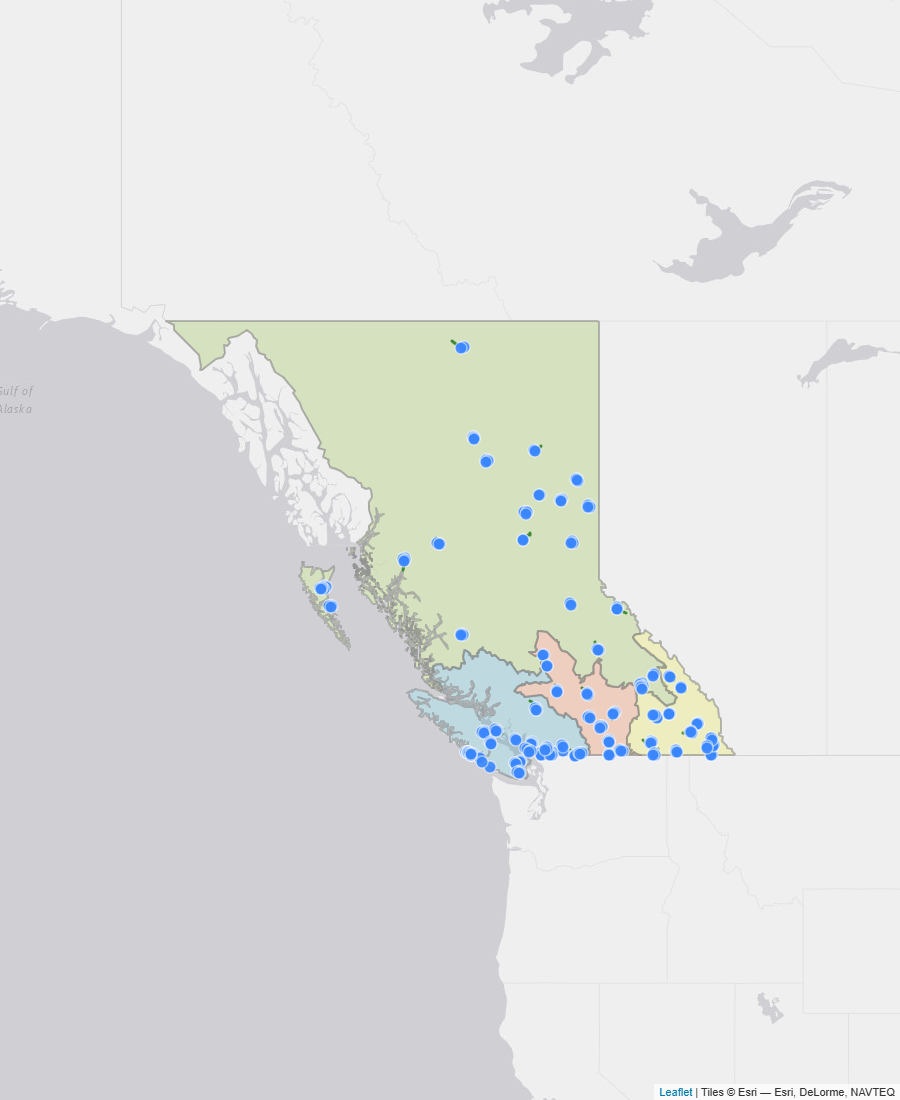
\includegraphics[width=3in,height=\textheight,keepaspectratio]{Figures/survey_map.png}

}

\caption{\label{fig-map}NABat survey efforts in 2025 within British
Columbia. Analysis regions were defined by Wildlife Conservation Society
Canada (WCSC) based on species ranges maps to group areas with similar
species compositions.}

\end{figure}%

\subsection{Activity Trend Models}\label{activity-trend-models}

Stationary data was used to estimate activity trends for 11 of BC's 15
resident species, while transect data was sufficient to estimate trends
for 9 species (Table~\ref{tbl-modelcov}). Of the stationary models,
seven species showed statistically significant positive trends (p
\textless{} 0.05):

\begin{itemize}
\item
  Townsend's Big-eared Bat (0.11 ± 0.05)
\item
  Big Brown Bat (0.07 ± 0.05)
\item
  Spotted Bat (0.12 ± 0.15)
\item
  Silver-haired Bat (0.04 ± 0.04)
\item
  California Myotis (0.01 ± 0.04)
\item
  Little Brown Mytois( 0.01 ± 0.04).
\item
  Long-legged Myotis (-0.00 ± 0.04).
\end{itemize}

No significant negative trends were detected in the stationary models.
The remaining species with sufficient data had non-significant trend
estimates.

Transect models yielded results for fewer species, with only Little
Brown Myotis showing a significant positive trend (0.16 ± 0.08). Trend
estimates for the remaining species with transect data were small and
non-significant.

\begin{table}[H]

\caption{\label{tbl-modelcov}Provincial stationary and transect trend
estimates from 2017-2024 NABat monitoring in BC adjusted for covariates.
Trends estimated on a logarithmic scale, thus a trend estimate of 0.05
corresponds to an annual change of 5\%. Significant results (p value
\textless{} 0.05) are highlighted in bold.}

\centering{

\centering
\begin{tabular}{l>{}r>{}r>{}r>{}r}
\toprule
\multicolumn{1}{c}{ } & \multicolumn{2}{c}{Stationary Models} & \multicolumn{2}{c}{Transect Models} \\
\cmidrule(l{3pt}r{3pt}){2-3} \cmidrule(l{3pt}r{3pt}){4-5}
Species & Trend Estimate ± 95\%CI & P-value & Trend Estimate ± 95\%CI & P-value\\
\midrule
Pallid Bat &  &  &  & \\
Townsend's Big-eared Bat & \textbf{0.11 ± 0.05} & \textbf{<0.001} &  & \\
Big Brown Bat & \textbf{0.07 ± 0.05} & \textbf{0.003} & 0.06 ± 0.09 & 0.150\\
Spotted Bat & 0.12 ± 0.15 & 0.114 &  & \\
Eastern Red Bat &  &  &  & \\
\addlinespace
Hoary Bat & 0.08 ± 0.20 & 0.441 & 0.01 ± 0.13 & 0.906\\
Silver-haired Bat & 0.04 ± 0.04 & 0.062 & 0.04 ± 0.07 & 0.311\\
California Myotis & 0.01 ± 0.04 & 0.632 & 0.06 ± 0.12 & 0.331\\
Western Small-footed Myotis &  &  & 0.22 ± 0.26 & 0.103\\
Long-eared Myotis & \textbf{0.09 ± 0.04} & \textbf{<0.001} & 0.04 ± 0.12 & 0.488\\
\addlinespace
Little Brown Myotis & 0.01 ± 0.04 & 0.544 & 0.16 ± 0.08 & \\
Northern Myotis &  &  &  & \\
Fringed Myotis & -0.00 ± 0.05 & 0.948 &  & \\
Long-legged Myotis & -0.00 ± 0.04 & 0.935 & 0.12 ± 0.14 & 0.094\\
Yuma Myotis & \textbf{0.08 ± 0.05} & \textbf{0.001} & 0.04 ± 0.15 & 0.582\\
\bottomrule
\end{tabular}

}

\end{table}%

Regional trend analyses revealed significant results (p \textless{}
0.05) across all regions with the most found in the South Coastal region
(Table~\ref{tbl-regionmodelcov}). Most significant results were
positive, but significant negative trends were found in:

\begin{itemize}
\item
  Hoary Bat in the South coastal Region (\textbf{-0.60 ± 0.58})
\item
  Yuma Myotis in the Northern Region (\textbf{-0.22 ± 0.22} ).
\end{itemize}

\begin{table}[H]

\caption{\label{tbl-regionmodelcov}Regional trend estimates from
2017-2024 NABat monitoring in BC adjusted for covariates. Trends
estimated on a logarithmic scale, thus a trend estimate of 0.05
corresponds to an annual change of 5\%. Significant results (p value
\textless{} 0.05) are highlighted in bold.}

\centering{

\fontsize{10.0pt}{13.0pt}\selectfont
\begin{tabular*}{\linewidth}{@{\extracolsep{\fill}}>{\raggedright\arraybackslash}p{\dimexpr 97.50pt -2\tabcolsep-1.5\arrayrulewidth}>{\centering\arraybackslash}p{\dimexpr 82.50pt -2\tabcolsep-1.5\arrayrulewidth}>{\centering\arraybackslash}p{\dimexpr 45.00pt -2\tabcolsep-1.5\arrayrulewidth}>{\centering\arraybackslash}p{\dimexpr 82.50pt -2\tabcolsep-1.5\arrayrulewidth}>{\centering\arraybackslash}p{\dimexpr 45.00pt -2\tabcolsep-1.5\arrayrulewidth}}
\toprule
 & \multicolumn{2}{>{\centering\arraybackslash}m{\dimexpr 127.50pt -2\tabcolsep-1.5\arrayrulewidth}}{\parbox{\linewidth}{\centering {Kootenay Region}}} & \multicolumn{2}{>{\centering\arraybackslash}m{\dimexpr 127.50pt -2\tabcolsep-1.5\arrayrulewidth}}{\parbox{\linewidth}{\centering {Northern Region}}} \\ 
\cmidrule(lr){2-3} \cmidrule(lr){4-5}
Species & Estimate ± 95\%CI & P-value & Estimate ± 95\%CI & P-value \\ 
\midrule\addlinespace[2.5pt]
Pallid Bat &  &  &  &  \\ 
Townsend's Big-eared Bat & 0.08 ± 0.10 & 0.118 &  &  \\ 
Big Brown Bat & 0.02 ± 0.12 & 0.707 & 0.02 ± 0.24 & 0.881 \\ 
Spotted Bat &  &  &  &  \\ 
Eastern Red Bat &  &  &  &  \\ 
Hoary Bat & 0.54 ± 0.59 & 0.073 & 1.05 ± 1.19 & 0.084 \\ 
Silver-haired Bat & \textbf{0.17 ± 0.08} & \textbf{<0.001} & 0.01 ± 0.14 & 0.882 \\ 
California Myotis & 0.03 ± 0.07 & 0.342 & 0.01 ± 0.11 & 0.829 \\ 
Western Small-footed Myotis &  &  &  &  \\ 
Long-eared Myotis & -0.02 ± 0.10 & 0.734 & 0.01 ± 0.15 & 0.934 \\ 
Little Brown Myotis & \textbf{0.11 ± 0.06} & \textbf{0.001} & -0.05 ± 0.09 & 0.308 \\ 
Northern Myotis &  &  &  &  \\ 
Fringed Myotis & -0.02 ± 0.14 & 0.828 &  &  \\ 
Long-legged Myotis & 0.06 ± 0.06 & 0.088 & -0.03 ± 0.11 & 0.617 \\ 
Yuma Myotis & -0.09 ± 0.15 & 0.222 & \textbf{-0.22 ± 0.22} & \textbf{0.043} \\ 
\bottomrule
\end{tabular*}

}

\end{table}%

\begin{table}
\fontsize{10.0pt}{13.0pt}\selectfont
\begin{tabular*}{\linewidth}{@{\extracolsep{\fill}}>{\raggedright\arraybackslash}p{\dimexpr 97.50pt -2\tabcolsep-1.5\arrayrulewidth}>{\centering\arraybackslash}p{\dimexpr 82.50pt -2\tabcolsep-1.5\arrayrulewidth}>{\centering\arraybackslash}p{\dimexpr 45.00pt -2\tabcolsep-1.5\arrayrulewidth}>{\centering\arraybackslash}p{\dimexpr 82.50pt -2\tabcolsep-1.5\arrayrulewidth}>{\centering\arraybackslash}p{\dimexpr 45.00pt -2\tabcolsep-1.5\arrayrulewidth}}
\toprule
 & \multicolumn{2}{>{\centering\arraybackslash}m{\dimexpr 127.50pt -2\tabcolsep-1.5\arrayrulewidth}}{\parbox{\linewidth}{\centering {Okanagan Region}}} & \multicolumn{2}{>{\centering\arraybackslash}m{\dimexpr 127.50pt -2\tabcolsep-1.5\arrayrulewidth}}{\parbox{\linewidth}{\centering {South Coastal Region}}} \\ 
\cmidrule(lr){2-3} \cmidrule(lr){4-5}
Species & Estimate ± 95\%CI & P-value & Estimate ± 95\%CI & P-value \\ 
\midrule\addlinespace[2.5pt]
Pallid Bat &  &  &  &  \\ 
Townsend's Big-eared Bat & 0.13 ± 0.14 & 0.067 & \textbf{0.20 ± 0.11} & \textbf{<0.001} \\ 
Big Brown Bat & 0.08 ± 0.14 & 0.279 & \textbf{0.21 ± 0.13} & \textbf{0.001} \\ 
Spotted Bat & 0.07 ± 0.16 & 0.375 & 0.23 ± 0.49 & 0.364 \\ 
Eastern Red Bat &  &  &  &  \\ 
Hoary Bat & -0.28 ± 0.63 & 0.379 & \textbf{-0.60 ± 0.58} & \textbf{0.044} \\ 
Silver-haired Bat & 0.05 ± 0.10 & 0.292 & 0.07 ± 0.10 & 0.180 \\ 
California Myotis & 0.06 ± 0.09 & 0.216 & \textbf{0.10 ± 0.07} & \textbf{0.004} \\ 
Western Small-footed Myotis &  &  &  &  \\ 
Long-eared Myotis & 0.03 ± 0.13 & 0.670 & 0.08 ± 0.10 & 0.123 \\ 
Little Brown Myotis & 0.04 ± 0.10 & 0.389 & \textbf{0.11 ± 0.08} & \textbf{0.008} \\ 
Northern Myotis &  &  &  &  \\ 
Fringed Myotis & -0.09 ± 0.13 & 0.195 & 0.16 ± 0.31 & 0.295 \\ 
Long-legged Myotis & \textbf{0.12 ± 0.11} & \textbf{0.034} & \textbf{0.09 ± 0.07} & \textbf{0.011} \\ 
Yuma Myotis & -0.10 ± 0.16 & 0.229 & \textbf{0.23 ± 0.12} & \textbf{<0.001} \\ 
\bottomrule
\end{tabular*}
\end{table}

\FloatBarrier

\subsection{Dynamic Occupancy Models}\label{dynamic-occupancy-models}

Across the 17 bat species modeled over the 9 years, no species showed a
clear decline in occupancy in BC. Several species showed increases, and
the rest were stable or showed too much uncertainty to draw conclusions
regarding trends (E.g., TABR, PAHE).

Species showing clear increases in occupancy (BC models): MYLU. MYEV,
MYVO, MYVU, MYCA, MYCI, LABO. LABO showed the strongest increase (0.22
to 0.59). MYLU was the most widespread species overall going from
\textasciitilde89\% to 97\% occupancy. Increases generally driven by
colonization rates exceeding extinction rates--bats showing up at sites
faster than they are leaving occupied ones.~

Species with stable or uncertain trends: EPFU, LACI, LANO, EUMA, COTO,
MYTH. ANPA is a special case-- showing a massive lambda value in the
BC-only model (and the BC + AK to some extent), but as per the note
below, this is mainly because of an artifact of going from near zero
occupancy to still-low occupancy, so the ratio is uncertain, reflected
by the wide credible intervals.~

Poorly estimated species: PAHE and TABR had extremely low detection
probabilities (0.5-0.7\%), leading to poor model convergence and very
wide credible intervals-interpret with caution or just state they are
data-deficient (models with that low of detection rates are basically
meaningless).~

Detection: Temperature was the most consistent detection
covariate--warmer nights equate to higher detection for most species.
There were some clutter effects on detection probability that were
species-specific. Julian date effects were mixed across species.~

\begin{figure}

\centering{

\pandocbounded{\includegraphics[keepaspectratio]{Figures/DOccupancy/ALL_occupancy_panel.png}}

}

\caption{\label{fig-dynamicocALL}Dynamic occupancy estimates (ψ) for 17
bat species monitored across British Columbia from 2017--2025. Points
represent annual mean occupancy estimates and shaded areas indicate 95\%
credible intervals.}

\end{figure}%

\section{Discussion}\label{discussion}

\subsection{Species Presence}\label{species-presence}

Species ranges across the project period (2016--2025) continue to appear
broadly stable, with no grid cells showing conspicuous or sustained
absences for previously detected species.

\subsection{Trend analyses}\label{trend-analyses}

\subsubsection{Activity Trends}\label{activity-trends-1}

Overall, results suggest that bat populations remain broadly stable
across British Columbia, with no species showing widespread negative
trends.

Several species showed statistically significant positive trends in both
province-wide and South Coastal regional models. However, these results
should be interpreted with caution. Caution is warranted when evaluating
the magnitude of the trend estimates. Several models exhibited
underdispersion, which, while not unexpected given the structural
characteristics of acoustic bat activity data, means that confidence
intervals and effect sizes should be interpreted carefully rather than
taken at face value.

The significant negative trend detected for Hoary Bat in the South
Coastal Region warrants attention and should be monitored closely in
coming years to determine whether this represents a genuine localized
decline or reflects sampling variability.

More broadly, as threats to bat populations continue to grow, it may be
worth exploring complementary analytical approaches alongside
activity-based trend models. Acoustic activity metrics carry inherent
noise, and detecting meaningful population signals can be challenging,
particularly for species with low detection rates or patchy
distributions. We recommend exploring occupancy modelling as a
complementary approach in future analyses, as it may provide a clearer
population signal by reducing the noise inherent in activity-based trend
estimates from stationary acoustic data.

\subsubsection{Dynamic Occupancy}\label{dynamic-occupancy-1}

The dynamic occupancy estimates suggest that the bat community in BC
appears to be generally stable to increasing over 2017-2025, with no
species showing evidence of decline. Species showing strongest increases
are Myotis species and LABO. Two species can't be reliably assessed
(PAHE, TABR) due to very low detection rates. Distance to road has an
effect on colonization and persistence dynamics for several species,
with sites closer to roads tending to have higher turnover.

\subsection{Challenges and Lessons
Learned}\label{challenges-and-lessons-learned}

\paragraph{\texorpdfstring{\textbf{Timing of Data Retrieval and
Submission}}{Timing of Data Retrieval and Submission}}\label{timing-of-data-retrieval-and-submission}

Field crews across British Columbia continue to reliably collect
recordings for their grid cells. However, organizing and submitting
these recordings, along with associated metadata, remains a challenge.
Delays in data submission from grid leaders extend processing and
analysis times, making it difficult to complete reports by the end of
the fiscal year. The transition in project management this year further
complicated data submission. We anticipate these challenges will be
resolved in future years as teams adjust to the new process. To improve
efficiency, we plan to increase reminders to grid leaders and provide
additional support to address ongoing challenges in data organization
and submission.

\subsection{Looking Forward}\label{looking-forward}

The BC NABat program has yielded a large and robust acoustic dataset
that provides solid baseline information on distribution and relative
abundance of 12 of 15 resident BC bat species. The data that has been
collected so far are an invaluable reference point for BC's bat
distributions and activity that improve with each additional year of
monitoring. Key considerations for the future of the program include:

\begin{itemize}
\item
  \textbf{Manual Verification Efficiency.} This was the first year that
  the BC monitoring program reduced the proportion of manual vetting
  carried out in the recordings to \textasciitilde50\% based on the
  findings from Stratton et al.~(2022). Careful consideration of these
  results compared to previous years will be considered as a guide for
  future models and analyses.
\item
  \textbf{Transect Sampling.} Transects are a relatively high
  labour/effort source of data than stationary detectors that require
  participants to work late into the night. They also often do not
  collect many recordings of bats in BC relative to the stationary
  detectors. However, transects are still the only source of reliable
  estimates of relative abundance. While continuing to support current
  transect sampling efforts, the NNW Bat Hub will work along side other
  partners to also explore other methods of creating reliable abundance
  estimates that are less labour intensive.
\item
  \textbf{Adding new grid cells.} Efforts will continue to be made to
  monitor as many of the same grid cells as possible, as the power of
  the dataset improves with each additional year. Moreover, looking for
  new opportunities to add new grid cells especially in under sampled
  regions of the province can help fill knowledge gaps for species
  distributions. New cells could also be added within ranges of species
  that are not widespread but easily monitored using acoustics. For
  example, Fringed Myotis and Spotted Bats are highly suited to acoustic
  surveillance, but only occur within a small portion of the grid cells
  being monitored currently
\end{itemize}

\newpage{}

\newpage{}

\section{Appendix A}\label{appendix-a}

Species and region specific dynamic occupancy results

\subsection{\texorpdfstring{Pallid Bat (\emph{Antrozous
pallidus)}}{Pallid Bat (Antrozous pallidus)}}\label{pallid-bat-antrozous-pallidus}

\pandocbounded{\includegraphics[keepaspectratio]{images/clipboard-3245689351.png}}\pandocbounded{\includegraphics[keepaspectratio]{images/clipboard-2058037231.png}}

\begin{figure}

\centering{

\pandocbounded{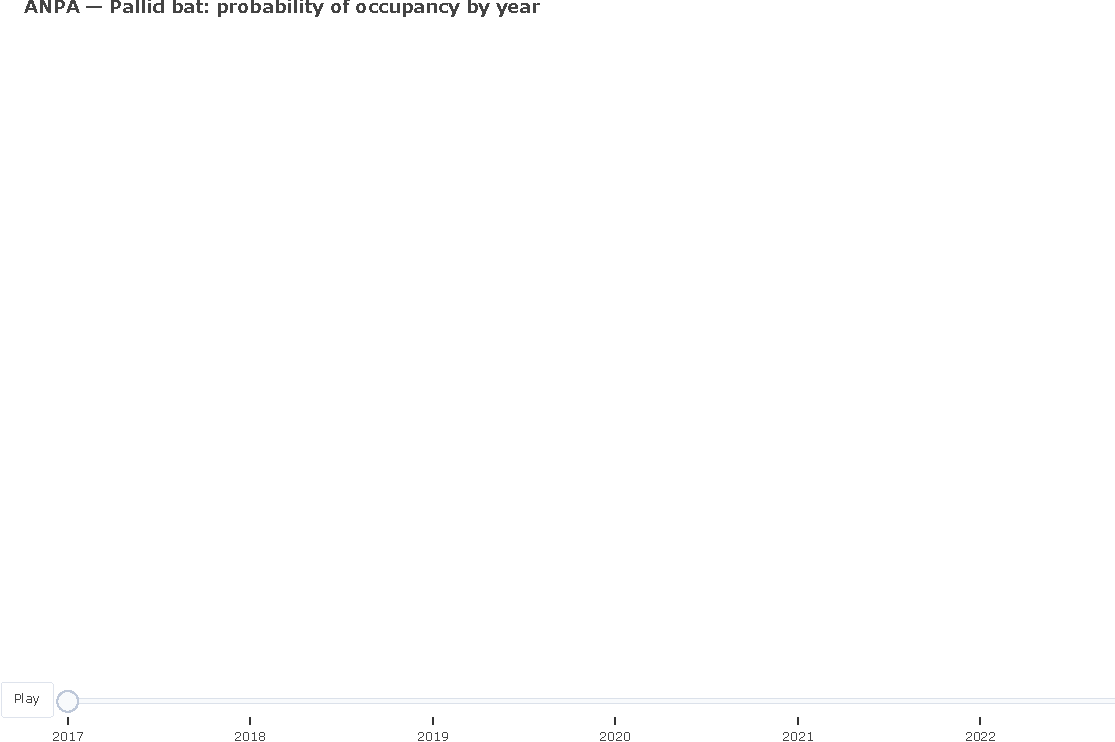
\includegraphics[keepaspectratio]{NABat-BC_2016-2025_files/figure-pdf/fig-occ-slider-anpa-1.pdf}}

}

\caption{\label{fig-occ-slider-anpa}Pallid bat (ANPA): probability of
occupancy per site by year. Circles = detected that year; triangles =
surveyed but not detected (colour is model inference); hollow grey = not
surveyed.}

\end{figure}%

\pandocbounded{\includegraphics[keepaspectratio]{images/clipboard-492828955.png}}\pandocbounded{\includegraphics[keepaspectratio]{images/clipboard-3792215063.png}}

\subsection{\texorpdfstring{Townsend's big-eared bat \emph{(Corynorhinus
townsendii})}{Townsend's big-eared bat (Corynorhinus townsendii)}}\label{townsends-big-eared-bat-corynorhinus-townsendii}

\pandocbounded{\includegraphics[keepaspectratio]{images/clipboard-2390708227.png}}\pandocbounded{\includegraphics[keepaspectratio]{images/clipboard-3771300722.png}}

\begin{figure}

\centering{

\pandocbounded{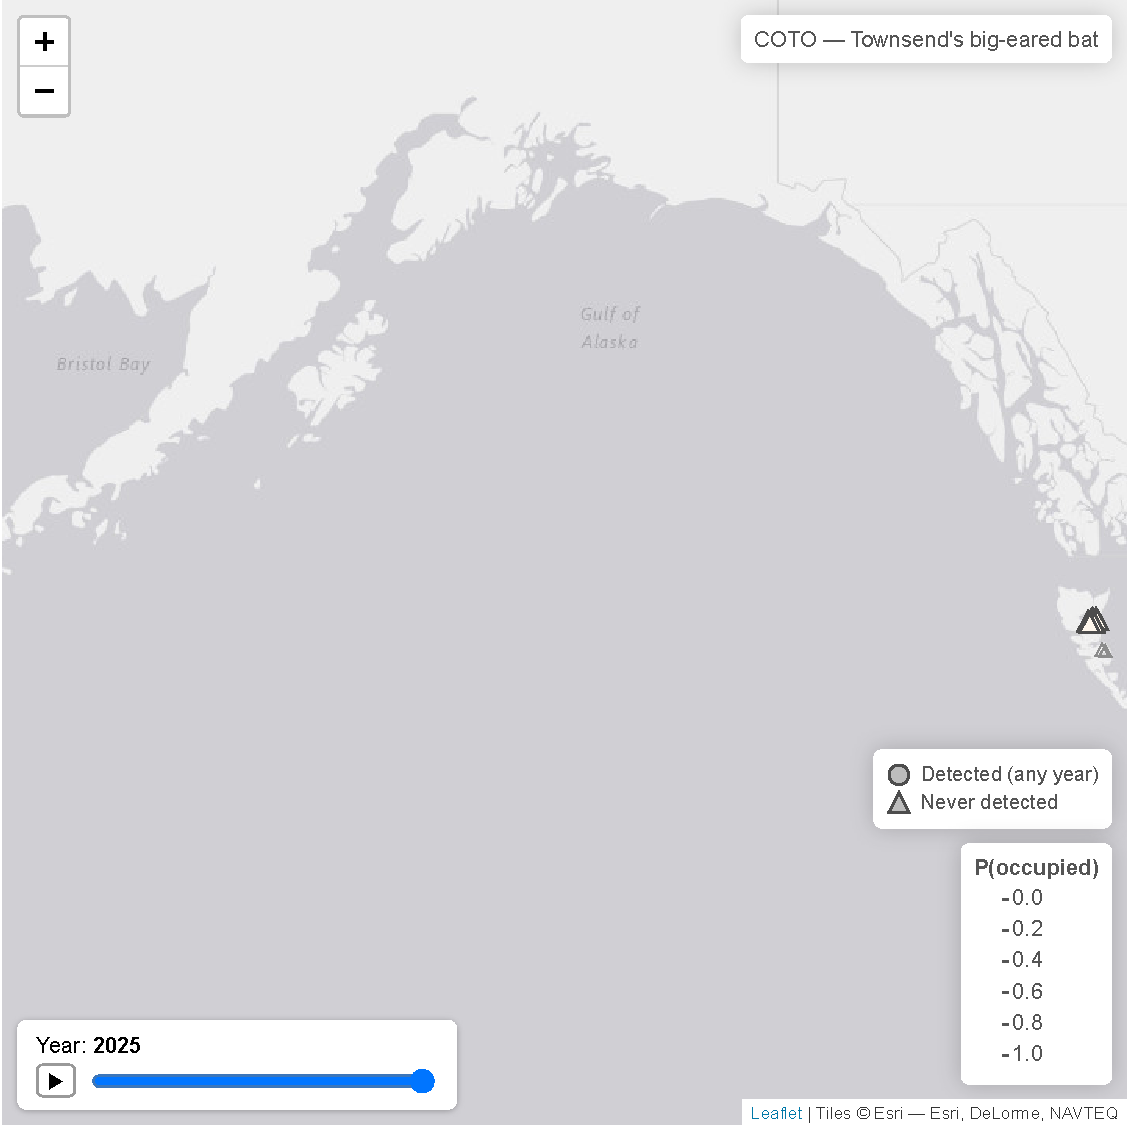
\includegraphics[keepaspectratio]{NABat-BC_2016-2025_files/figure-pdf/fig-occ-slider-COTO-1.pdf}}

}

\caption{\label{fig-occ-slider-COTO}Townsend's big-eared bat (COTO):
probability of occupancy per site by year. Circles = detected that year;
triangles = surveyed but not detected (colour is model inference);
hollow grey = not surveyed.}

\end{figure}%

\pandocbounded{\includegraphics[keepaspectratio]{images/clipboard-2446265377.png}}\pandocbounded{\includegraphics[keepaspectratio]{images/clipboard-1492990181.png}}

\subsection{\texorpdfstring{Big brown bat (\emph{Eptesicus
fuscus})}{Big brown bat (Eptesicus fuscus)}}\label{big-brown-bat-eptesicus-fuscus}

\pandocbounded{\includegraphics[keepaspectratio]{images/clipboard-1583198714.png}}\pandocbounded{\includegraphics[keepaspectratio]{images/clipboard-2529446978.png}}\pandocbounded{\includegraphics[keepaspectratio]{images/clipboard-3997919441.png}}\pandocbounded{\includegraphics[keepaspectratio]{images/clipboard-446568693.png}}

\subsection{\texorpdfstring{Spotted bat (\emph{Euderma
maculatum})}{Spotted bat (Euderma maculatum)}}\label{spotted-bat-euderma-maculatum}

\section*{Literature Cited}\label{literature-cited}
\addcontentsline{toc}{section}{Literature Cited}

\protect\phantomsection\label{refs}
\begin{CSLReferences}{1}{1}
\bibitem[\citeproctext]{ref-cwhc-rcsf2024Canadian}
CWHC-RCSF. 2024. {``Canadian {Wildlife Health Cooperative} - {Réseau}
Canadien Pour La Santé de La Faune.''}
\url{https://www.cwhc-rcsf.ca/white_nose_syndrome_reports_and_maps.php}.

\bibitem[\citeproctext]{ref-ministryofenergyandclimatesolutions2024BC}
Energy and Climate Solutions, Ministry of. 2024. {``{BC Gov News}.''}
December 9. \url{https://news.gov.bc.ca/releases/2024ECS0048-001643}.

\bibitem[\citeproctext]{ref-friedenberg2021Assessing}
Friedenberg, Nicholas A., and Winifred F. Frick. 2021. {``Assessing
Fatality Minimization for Hoary Bats Amid Continued Wind Energy
Development.''} \emph{Biological Conservation} 262 (October): 109309.
\url{https://doi.org/10.1016/j.biocon.2021.109309}.

\bibitem[\citeproctext]{ref-loeb2015Plan}
Loeb, Susan C., Thomas J. Rodhouse, Laura E. Ellison, et al. 2015.
\emph{A Plan for the {North American Bat Monitoring Program} ({NABat})}.
SRS-GTR-208. U.S. Department of Agriculture, Forest Service, Southern
Research Station. \url{https://doi.org/10.2737/SRS-GTR-208}.

\bibitem[\citeproctext]{ref-olsonBat}
Olson, Cory. n.d. {``Bat {Profiles}.''} Alberta Community Bat Program.
Accessed March 6, 2025. \url{https://www.albertabats.ca/batprofiles/}.

\bibitem[\citeproctext]{ref-rae2022North}
Rae, Jason, and Cori L Lausen. 2022. \emph{North {American Bat
Monitoring Program} in {British Columbia}: 2021 {Data Summary} and
{Activity Trend Analyses} (2016-2021).} Wildlife Conservation Society of
Canada.

\bibitem[\citeproctext]{ref-rae2024North}
Rae, Jason, and Cori L Lausen. 2024. \emph{North {American Bat
Monitoring Program} in {British Columbia}: 2023 {Data Summary} and
{Activity Trend Analyses} (2016-2023).} Wildlife Conservation Society of
Canada.

\bibitem[\citeproctext]{ref-reichert2018Guide}
Reichert, Brian, Cori Lausen, Susan Loeb, et al. 2018. \emph{A {Guide}
to {Processing Bat Acoustic Data} for the {North American Bat Monitoring
Program} ({NABat})}. Open-File Nos. 2018--1068. U.S. Geological Survey.

\bibitem[\citeproctext]{ref-slough2022New}
Slough, Brian, Cori Lausen, Brian Paterson, et al. 2022. {``New Records
about the Diversity, Distribution, and Seasonal Activity Patterns by
Bats in {Yukon} and Northwestern {British Columbia}.''}
\emph{Northwestern Naturalist} 103 (August): 162--82.
\url{https://doi.org/10.1898/NWN21-10}.

\bibitem[\citeproctext]{ref-solick2022Bat}
Solick, Donald. 2022. {``Bat {Acoustic Species-Pair Matrix Western
US}/{Canada}.''}
\url{https://www.batacousticsurveys.com/_files/ugd/a1e0ca_0ed9c3172b9145e49c50eb7a7712f909.pdf}.

\bibitem[\citeproctext]{ref-committeeonthestatusofendangeredwildlifeincanada2023Hoary}
Status of Endangered Wildlife in Canada, Committee on the. 2023.
{``Hoary {Bat} ({Lasiurus} Cinereus) {Eastern Red Bat} ({Lasiurus}
Borealis) {Silver-haired Bat} ({Lasionycteris} Noctivagans): {COSEWIC}
Assessment and Status Report 2023.''}
\url{https://www.canada.ca/en/environment-climate-change/services/species-risk-public-registry/cosewic-assessments-status-reports/hoary-bat-eastern-red-bat-silver-haired-bat-2023.html}.

\bibitem[\citeproctext]{ref-stratton2022Coupling}
Stratton, Christian, Kathryn M. Irvine, Katharine M. Banner, Wilson J.
Wright, Cori Lausen, and Jason Rae. 2022. {``Coupling Validation Effort
with in Situ Bioacoustic Data Improves Estimating Relative Activity and
Occupancy for Multiple Species with Cross‐species Misclassifications.''}
\emph{Methods in Ecology and Evolution} 13 (6): 1288--303.
\url{https://doi.org/10.1111/2041-210X.13831}.

\bibitem[\citeproctext]{ref-szewczak2018Acoustic}
Szewczak, Joe. 2018. \emph{Acoustic {Features} of {Western US Bats}}.
Humboldt State University Bat Lab.

\bibitem[\citeproctext]{ref-BCBatAction2024Plan}
Team, BC Bat Action. 2024. \emph{2024-2028 BC Bat Action Plan}.

\bibitem[\citeproctext]{ref-u.s.fishandwidlifeserviceusfws2025WhiteNose}
USFWS, U. S. Fish and Widlife Service. 2025. {``White-{Nose
Syndrome}.''} \url{https://www.whitenosesyndrome.org/}.

\bibitem[\citeproctext]{ref-zimmerling2016Bat}
Zimmerling, J. Ryan, and Charles M. Francis. 2016. {``Bat Mortality Due
to Wind Turbines in {Canada}.''} \emph{The Journal of Wildlife
Management} 80 (8): 1360--69. \url{https://doi.org/10.1002/jwmg.21128}.

\end{CSLReferences}




\end{document}
